% Build this document with LuaTeX, a modern Unicode-aware LaTeX engine
% that uses system TTF and OTF font files.
% This is needed for the fontspec, microtype, and nolig packages.

\newcommand{\bodyfontsize}{10bp}
\newcommand{\bodybaselineskip}{12bp}

\RequirePackage[table]{xcolor}

% We're using KOMA Script to hand-tune footnotes and TOC appearance.
% It should be available in your texlive distribution,
% which is how most distros package LaTeX.
\documentclass[fontsize=10pt, oneside]{scrartcl}

% Margins: see http://practicaltypography.com/page-margins.html and
% http://practicaltypography.com/line-length.html
% We're aiming for 80-ish characters per line.
\usepackage[
    letterpaper,
    footnotesep=\bodybaselineskip,
    left=0.75in,right=0.75in,top=1in,bottom=1in,
]{geometry}

% Font specification.
\usepackage[no-math]{fontspec}
\usepackage[fleqn]{amsmath}

\usepackage[italic]{mathastext}

\usepackage{polyglossia}
\setdefaultlanguage[variant=american]{english}

\usepackage{microtype} % Font expansion, protrusion, and other goodness

% Disable ligatures across grapheme boundaries
% (see the package manual for details.)
\usepackage[english]{selnolig}

% Use symbols for footnotes, resetting each page
\usepackage[perpage,bottom,symbol*]{footmisc}

% Don't use a sans font for description labels.
\addtokomafont{descriptionlabel}{\rmfamily\mdseries}
\setkomafont{disposition}{\rmfamily}
\setkomafont{section}{\large\itshape}
\setkomafont{subsection}{\normalsize\itshape}
\renewcommand*\thesection{\upshape\arabic{section}}

% Use uppercase numbers for numbered lists.
% (We're using lowercase ones for the body text.)
% See http://tex.stackexchange.com/a/133186
\usepackage{enumitem}
\setlist[enumerate]{font=\addfontfeatures{Numbers=LowercaseOff}}

% Custom footer
\usepackage{scrlayer-scrpage}
\setkomafont{pagefoot}{\sffamily\upshape}
\pagestyle{scrheadings}

\usepackage{minted} % Syntax highlighting via Pygments
\usemintedstyle{friendly}

\usepackage{graphicx}
\usepackage[font=footnotesize,justification=raggedright]{caption}

\usepackage{tikz} % Duck and cover.

\newcommand{\codesize}{\fontsize{\bodyfontsize}{\bodybaselineskip}}

% Syntax highlighting for ARM asm (minted doesn't do this well)
\usepackage{listings}
\lstset{
basicstyle=\ttfamily\codesize\selectfont,
keywordstyle=\color{darkGreen}\bfseries,
commentstyle=\textcolor[rgb]{0.25,0.50,0.50}
}
% listings definitions for ARM assembly.
% Get them from https://github.com/frosc/arm-assembler-latex-listings,
% install as shown at http://tex.stackexchange.com/a/1138/92465
\usepackage{lstlangarm} % See above

\usepackage{changepage} % For adjustwidth

\usepackage{metalogo} % for \LuaLaTeX

\setlength\columnsep{2em}
%\setlength\parskip{0em}
\setlength\parindent{1.5em}

\title{Concurrency Primer\footnote{The original title was "What every systems programmer should know about concurrency."}}
\author{Matt Kline and Ching-Chun (Jim) Huang}
\date{\today}

% Custom footer
% Hyperlinks
\usepackage[unicode,pdfusetitle]{hyperref}
\usepackage{xcolor}
\definecolor{darkGreen}{HTML}{008000}
\hypersetup{
    colorlinks=true, % Use colors
    linkcolor=violet, % Intra-doc links
    urlcolor=blue % URLs are blue
}

% Use \punckern to overlap periods, commas, and footnote markers
% for a tighter look.
% Care should be taken to not make it too tight - f" and the like can overlap
% if you're not careful.
\newcommand{\punckern}{\kern-0.4ex}
% For placing commas close to, or under, quotes they follow.
% We're programmers, and we blatantly disregard American typographical norms
% to put the quotes inside, but we can at least make it look a bit nicer.
\newcommand{\quotekern}{\kern-0.5ex}


% Create an unbreakable string of text in a monospaced font.
% Useful for `command --line --args`
\newcommand{\monobox}[1]{\mbox{\texttt{#1}}}

\newcommand{\keyword}[1]{\monobox{\color{darkGreen}#1}}

% C++ looks nicer if the ++ is in a monospace font and raised a bit.
% Also, use uppercase numbers to match the capital C.
\newcommand{\cplusplus}[1]{C\kern-0.1ex\raisebox{0.15ex}{\texttt{++}}{\addfontfeature{Numbers=LowercaseOff}#1}}
\newcommand{\clang}[1]{C{\addfontfeature{Numbers=LowercaseOff}#1}}
\newcommand{\csharp}{C\raisebox{0.25ex}{\#}}

\newcommand{\fig}[1]{Figure~\ref{#1}}

% Italicize new terms
\newcommand{\introduce}[1]{\textit{#1}}

\newcommand{\secref}[1]{\hyperref[#1]{\textsc{\S}\ref*{#1}}}

% Feel free to futz with the spacing above and below these.
% (Given the number of code snippets and figures,
% they can really make or break the spacing of the paragraphs.
% Keep in mind that TeX only lays out a page at a time,
% so you need to more or less look at how each page is individually handled.
\newenvironment{colfigure}
  {\par\vspace{1\baselineskip minus 0.5\baselineskip}\noindent\minipage{\linewidth}}
  {\endminipage\vspace{1\baselineskip minus 0.7\baselineskip}}

% See http://tex.stackexchange.com/a/68310
\makeatletter
\let\runauthor\@author
\let\rundate\@date
\let\runtitle\@title
\makeatother

% Spend a bit more time to get better word spacing.
% See http://tex.stackexchange.com/a/52855/92465
\emergencystretch=1em

\begin{document}
% Custom title instead of \maketitle
\begin{center}
\Large \runtitle
\bigskip

\large
\runauthor
\smallskip

\normalsize
\rundate
\end{center}
\bigskip

\begin{center}
\large \bfseries\itshape Abstract
\end{center}
\smallskip

\noindent
System programmers are acquainted with tools such as mutexes, semaphores, and condition variables.
However, the question remains: how do these tools work, and how do we write concurrent code in their absence?
For example, when working in an embedded environment beneath the operating system,
or when faced with hard time constraints that prohibit blocking.
Furthermore, since the compiler and hardware often combine to transform code into an unanticipated order,
how do multithreaded programs work? Concurrency is a complex and counterintuitive topic,
but let us endeavor to explore its fundamental principles.
\bigskip

\section{Background}
\label{background}

Modern computers run many instruction streams concurrently.
On single-core machines, they take turns, sharing the \textsc{cpu} in short slices of time.
On multi-core machines, several can run in parallel.
We call them many names---processes, threads, tasks, interrupt service routines (ISR),
and more---but most of the same principles apply across the board.

While computer scientists have created many excellent abstractions, ultimately,
these instruction streams (let's refer to them as ``\emph{threads}`` for the sake of brevity) interact by sharing bits of state.
For this to work correctly, we must understand the order in which threads read and write to memory.
Consider a straightforward example in which thread \textit{A} shares an integer with others.
It writes the integer to a variable and then sets a flag to instruct other threads to read whatever it has just stored.
As code, this might resemble:
\begin{colfigure}
\begin{minted}[fontsize=\codesize]{c}
int v;
bool v_ready = false;

void threadA()
{
    // Write the value
    // and set its ready flag.
    v = 42;
    v_ready = true;
}
\end{minted}
\end{colfigure}
\begin{colfigure}
\begin{minted}[fontsize=\codesize]{c}
void threadB()
{
    // Await a value change and read it.
    while (!v_ready) { /* wait */ }
    const int my_v = v;
    // Do something with my_v...
}
\end{minted}
\end{colfigure}
We must ensure that other threads only observe \textit{A}'s write to \texttt{v\_ready} \emph{after A's} write to \texttt{v}.
If another thread can ``see'' \texttt{v\_ready} becoming true before observing \texttt{v} becoming $42$,
this simple scheme will not work correctly.

You would think it is trivial to guarantee this order, but nothing is as it seems.
For starters, any optimizing compiler will rewrite your code to run faster on the hardware it is targeting.
As long as the resulting instructions run to the same effect \emph{for the current thread},
reads and writes can be moved to avoid pipeline stalls\footnote{%
Most \textsc{cpu} designs execute parts of several instructions in parallel to increase their throughput (see \fig{pipeline}).
When the result of one instruction is needed by a subsequent instruction in the pipeline,
the \textsc{cpu} may need to suspend forward progress or \introduce{stall} until that result is ready.}
or improve locality.\punckern\footnote{%
\textsc{ram} is not read in single bytes, but in chunks called \introduce{cache lines}.
If variables that are used together can be placed on the same cache line,
they will be read and written all at once.
This usually provides a massive speedup,
but as we will see in \secref{false-sharing},
can bite us when a line must be shared between cores.}

Variables can be assigned to the same memory location if they are never used at the same time.
Calculations can be made speculatively before a branch is taken,
then ignored if the compiler guessed incorrectly.\punckern\footnote{%
This is especially common when using profile-guided optimization (PGO).}
%(These sorts of optimizations  sometimes called the ``as-if'' rule in \cplusplus{}.)

Even if the compiler did not change our code,
we would still be in trouble since our hardware does it too!
A modern \textsc{cpu} processes instructions in a \emph{much} more complicated fashion than traditional pipelined approaches like the one shown in \fig{pipeline}.
They contain many data paths, each for different types of instructions,
and schedulers which reorder and route instructions through these paths.
\begin{colfigure}
  \centering
  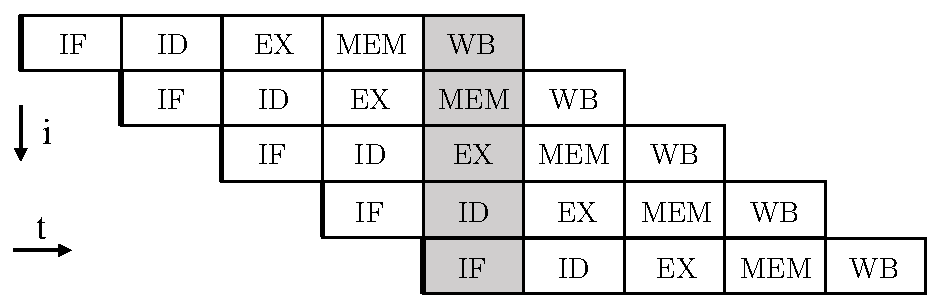
\includegraphics[keepaspectratio,width=0.7\linewidth]{images/pipeline}
  \captionof{figure}{A traditional five-stage \textsc{cpu} pipeline with fetch, decode, execute, memory access, and write-back stages.
                     Modern designs are much more complicated, often reordering instructions on the fly.}
  \label{pipeline}
\end{colfigure}

It is also easy to make naive assumptions about how memory works.
If we imagine a multi-core processor, we might think of something resembling \fig{ideal-machine},
where each core takes turns performing reads and writes to the system's memory.
\begin{colfigure}
\centering
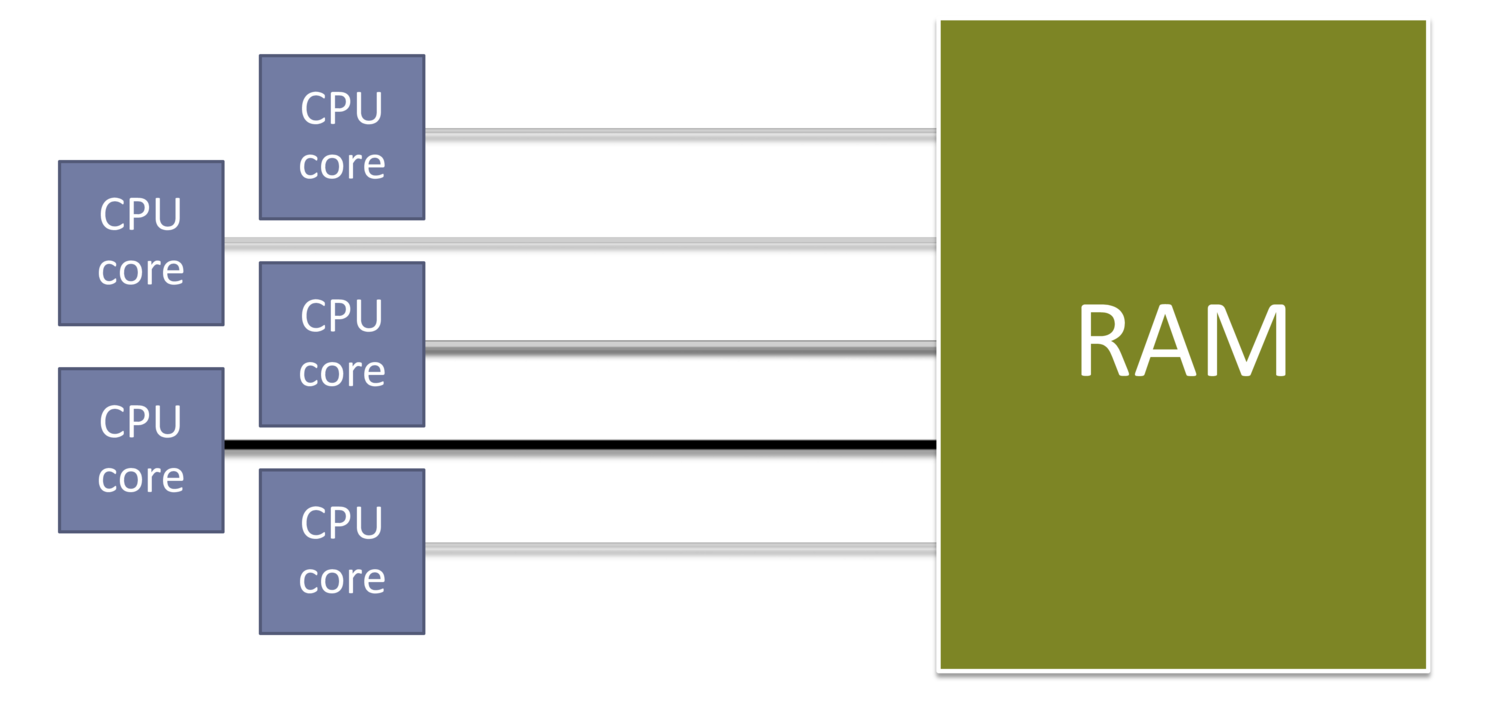
\includegraphics[keepaspectratio, width=0.8\linewidth]{ideal-machine}
\captionof{figure}{An idealized multi-core processor where cores
take turns accessing a single shared set of memory.}
\label{ideal-machine}
\end{colfigure}
But the world is not so simple.
While processor speeds have increased exponentially over the past decades,
\textsc{ram} hasn't been able to keep up,
creating an ever-widening gulf between the time it takes to run an
instruction and the time needed to retrieve its data from memory.
Hardware designers have compensated by placing a growing number of
hierarchical caches directly on the \textsc{cpu} die.
Each core also usually has a \introduce{store buffer} that handles
pending writes while subsequent instructions are executed.
Keeping this memory system \introduce{coherent},
so that writes made by one core are observable by others,
even if those cores use different caches, is quite challenging.

\begin{colfigure}
  \centering
  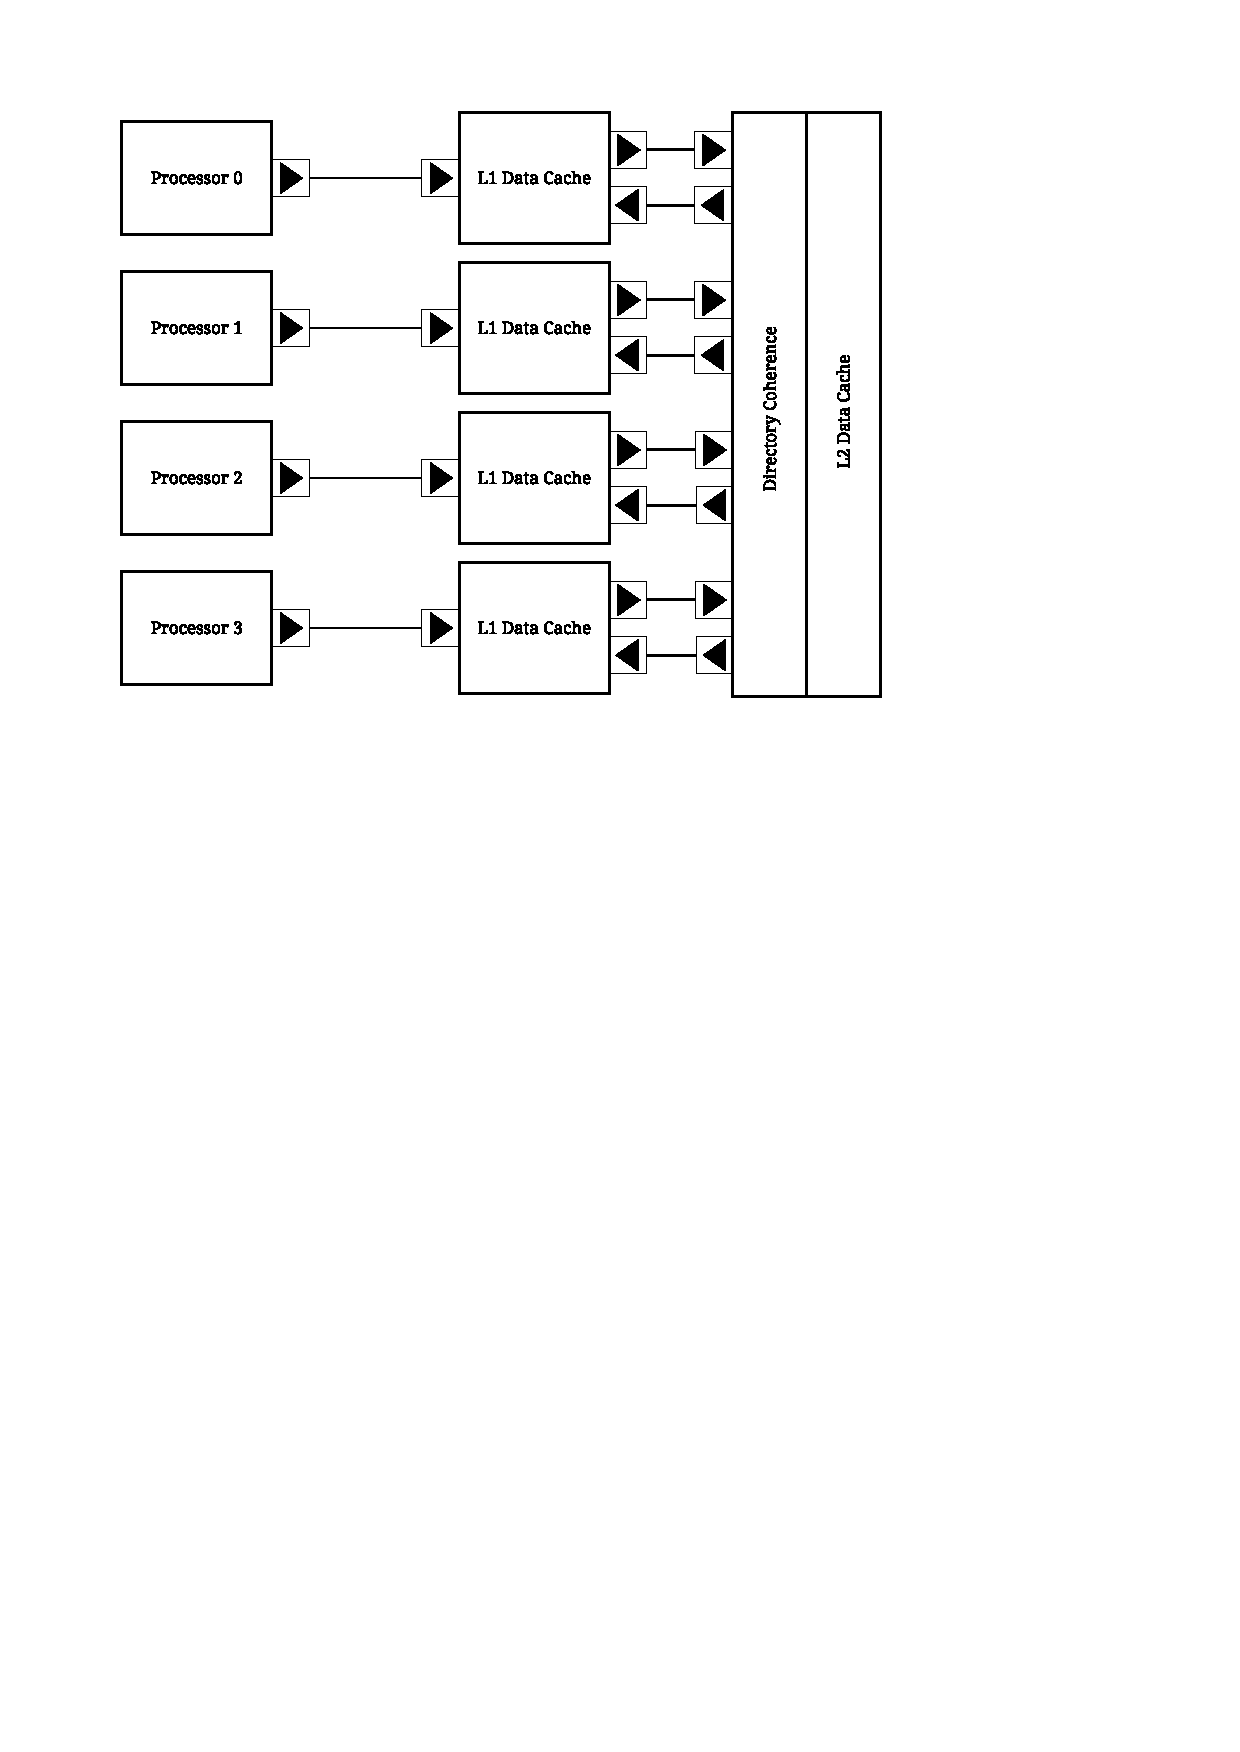
\includegraphics[keepaspectratio, width=0.8\linewidth]{images/mp-cache}
  \captionof{figure}{A common memory hierarchy for modern multi-core processors}
  \label{dunnington}
\end{colfigure}

All of these complexities mean that there is no consistent concept of ``now'' in a multithreaded program,
especially on a multi-core c\textsc{cpu}.
Creating some sense of order between threads is a collaborative effort of the hardware,
the compiler, the programming language, and your application.
Let's explore what we can do and what tools we will need.

\section{Enforcing law and order}
\label{seqcst}

Creating order in multithreaded programs requires different approaches on each \textsc{cpu} architecture.
For many years, systems languages like \clang{} and \cplusplus{} had no notion of concurrency,
forcing developers to use assembly or compiler extensions.
This was finally fixed in 2011, when both languages' \textsc{iso} standards added synchronization tools.
So long as you use them correctly,
the compiler will prevent any reorderings---both by its own optimizer,
and by the \textsc{cpu}---that cause data races.\punckern\footnote{%
The ISO~\clang{11} standard lifted its concurrency facilities,
almost verbatim, from the \cplusplus{11} standard.
Everything you see here should be identical in both languages, barring some arguably cleaner syntax in \cplusplus{}.
}

Let's try our previous example again.
For it to work, the ``ready'' flag needs to use an \introduce{atomic type}.
\begin{colfigure}
\begin{minted}[fontsize=\codesize]{c}
#include <stdatomic.h>
int v = 0;
atomic_bool v_ready = false;

void *threadA() {
    v = 42;
    v_ready = true;
}
\end{minted}
\end{colfigure}
\begin{colfigure}
\begin{minted}[fontsize=\codesize]{c}
int bv;

void *threadB() {
    while(!v_ready) { /* wait */ }
    bv = v;
    /* Do something */
}
\end{minted}
\end{colfigure}
The \clang{} and \cplusplus{} standard libraries define a series of these types in \mintinline{c}{<stdatomic.h>} and \mintinline{cpp}{<atomic>},
respectively.
They look and act just like the integer types they mirror (e.g., \monobox{bool}~\textrightarrow~\monobox{atomic\_bool},
\monobox{int}~\textrightarrow~\monobox{atomic\_int}, etc.),
but the compiler ensures that other variables' loads and stores are not reordered around theirs.

Informally, we can think of atomic variables as rendezvous points for threads.
By making \monobox{v\_ready} atomic,
\monobox{v = 42}\, is now guaranteed to happen before \monobox{v\_ready = true}\, in thread~\textit{A},
just as \monobox{my\_v = v}\, must happen after reading \monobox{v\_ready}\,
in thread~\textit{B}.
Formally, atomic types establish a \textit{single total modification order} where,
``[\ldots] the result of any execution is the same as if the reads and writes occurred in some order, and the operations of each individual processor appear in this sequence in the order specified by its program.''
This model, defined by Leslie Lamport in 1979,
is called \introduce{sequential consistency}.

\section{Atomicity}
\label{atomicity}
But order is only one of the vital ingredients for inter-thread communication.
The other is what atomic types are named for: atomicity.
Something is \introduce{atomic} if it can not be divided into smaller parts.
If threads do not use atomic reads and writes to share data, we are still in trouble.

Consider a program with two threads.
One thread processes a list of files, incrementing a counter each time it finishes working on one.
The other thread handles the user interface, periodically reading the counter to update a progress bar.
If that counter is a 64-bit integer, we can not access it atomically on 32-bit machines,
since we need two loads or stores to read or write the entire value.
If we are particularly unlucky, the first thread could be halfway through writing the counter when the second thread reads it,
receiving garbage.
These unfortunate occasions are called \introduce{torn reads and writes}.

If reads and writes to the counter are atomic, however, our problem disappears.
We can see that, compared to the difficulties of establishing the right order,
atomicity is fairly straightforward:
just make sure that any variables used for thread synchronization
are no larger than the \textsc{cpu} word size.

\section{Arbitrarily-sized “atomic” types}

Along with \texttt{atomic\_int} and friends,
\cplusplus{} provides the template \texttt{std::atomic<T>} for defining arbitrary atomic types.
\clang{}, lacking a similar language feature but wanting to provide the same functionality,
added an \keyword{\_Atomic} keyword.
If \texttt{T} is larger than the machine's word size,
the compiler and the language runtime automatically surround the variable's reads and writes with locks.
If you want to make sure this is not happening,\punckern\footnote{%
\ldots which is most of the time,
since we are usually using atomic operations to avoid locks in the first place.}
you can check with:
\begin{colfigure}
\begin{minted}[fontsize=\codesize]{cpp}
std::atomic<Foo> bar;
ASSERT(bar.is_lock_free());
\end{minted}
\end{colfigure}
In most cases,\punckern\footnote{%
The language standards permit atomic types to be \emph{sometimes} lock-free.
This might be necessary for architectures that do not guarantee atomicity for unaligned reads and writes.}
this information is known at compile time.
Consequently, \cplusplus{17} added \texttt{is\_always\_lock\_free}:
\begin{colfigure}
\begin{minted}[fontsize=\codesize]{cpp}
static_assert(
  std::atomic<Foo>::is_always_lock_free);
\end{minted}
\end{colfigure}

\section{Read-modify-write}
\label{rmw}

Loads and stores are all well and good,
but sometimes we need to read a value, modify it,
and write it back as a single atomic step.
There are a few common \introduce{read-modify-write} \textsc{(rmw)} operations.
In \cplusplus{}, they are represented as member functions of \texttt{std::atomic<T>}.
In \clang{}, they are freestanding functions.

\subsection{Exchange}
\label{exchange}

The simplest atomic \textsc{rmw} operation is an \introduce{exchange}:
the current value is read and replaced with a new one.
To see where this might be useful,
let's tweak our example from \secref{atomicity}:
instead of displaying the total number of processed files,
the \textsc{ui} might want to show how many were processed per second.
We could implement this by having the \textsc{ui} thread read the counter then zero it each second.
But we could get the following race condition if reading and zeroing are separate steps:
\begin{enumerate}
\item The \textsc{ui} thread reads the counter.
\item Before the \textsc{ui} thread has the chance to zero it,
      the worker thread increments it again.
\item The \textsc{ui} thread now zeroes the counter, and the previous increment
      is lost.
\end{enumerate}
If the \textsc{ui} thread atomically exchanges the current value with zero,
the race disappears.

\subsection{Test and set}

\introduce{Test-and-set} works on a Boolean value:
we read it, set it to \mintinline{cpp}{true}, and provide the value it held beforehand.
\clang{} and \cplusplus{} offer a type dedicated to this purpose, called \monobox{atomic\_flag}.
We could use it to build a simple spinlock:
\label{spinlock}
\begin{colfigure}
\begin{minted}[fontsize=\codesize]{cpp}
atomic_flag af = ATOMIC_FLAG_INIT;

void lock()
{
    while (atomic_flag_test_and_set(&af)) { /* wait */ }
}

void unlock() { atomic_flag_clear(&af); }
\end{minted}
\end{colfigure}
If we call \mintinline{cpp}{lock()} and the previous value is \mintinline{cpp}{false},
we are the first to acquire the lock,
and can proceed with exclusive access to whatever the lock protects.
If the previous value is \mintinline{cpp}{true},
someone else has acquired the lock and we must wait until they release it by clearing the flag.

\subsection{Fetch and…}

We can also read a value,
perform some simple operation on it (addition, subtraction, bitwise \textsc{and}, \textsc{or}, \textsc{xor}),
and return its previous value---all as one atomic operation.
You might have noticed in the exchange example that the worker thread's additions must also be atomic,
or else we could get a race where:
\begin{enumerate}
\item The worker thread loads the current counter value and adds one.
\item Before that thread can store the value back,
      the \textsc{ui} thread zeroes the counter.
\item The worker now performs its store, as if the counter was never cleared.
\end{enumerate}

\subsection{Compare and swap}
\label{cas}

Finally, we have \introduce{compare-and-swap} \textsc{(cas)},
sometimes called \introduce{compare-and-exchange}.
It allows us to conditionally exchange a value \emph{if} its previous value matches some expected one.
In \clang{} and \cplusplus{}, \textsc{cas} resembles the following,
if it were executed atomically:
\begin{colfigure}
\begin{minted}[fontsize=\codesize]{cpp}
template <typename T>
bool atomic<T>::compare_exchange_strong(
    T& expected, T desired)
{
    if (*this == expected) {
        *this = desired;
        return true;
    }
    expected = *this;
    return false;
}
\end{minted}
\end{colfigure}

\begin{samepage}
\noindent You might be perplexed by the \texttt{\_strong} suffix.
Is there a ``weak'' \textsc{cas}?
Yes, but hold onto that thought---we'll talk about it in \secref{spurious-ll/sc-failures}.
\end{samepage}

Let's say we have some long-running task that we might want to cancel.
We'll give it three states: \textit{idle}, \textit{running},
and \textit{cancelled}, and write a loop that exits when it is cancelled.
\begin{colfigure}
\begin{minted}[fontsize=\codesize]{cpp}
enum class TaskState : int8_t {
    Idle, Running, Cancelled
};

std::atomic<TaskState> ts;

void taskLoop()
{
    ts = TaskState::Running;
    while (ts == TaskState::Running) {
      // Do good work.
    }
}
\end{minted}
\end{colfigure}
If we want to cancel the task if it is running, but do nothing if it is idle,
we could \textsc{cas}:
\begin{colfigure}
\begin{minted}[fontsize=\codesize]{cpp}
bool cancel()
{
    auto expected = TaskState::Running;
    return ts.compare_exchange_strong(expected, TaskState::Cancelled);
}
\end{minted}
\end{colfigure}

\section{Atomic operations as building blocks}

Atomic loads, stores, and \textsc{rmw} operations are the building blocks for every single concurrency tool.
It is useful to split those tools into two camps:
\introduce{blocking} and \introduce{lockless}.

Blocking synchronization methods are usually simpler to reason about,
but they can make threads pause for arbitrary amounts of time.
For example, consider a mutex,
which forces threads to take turns accessing shared data.
If some thread locks the mutex and another tries to do the same,
the second thread must wait---or \introduce{block}---until the first thread releases the lock,
however long that may be.
Blocking mechanisms are also susceptible to \introduce{deadlock} and \introduce{livelock}---
bugs where the entire system ``gets stuck'' due to threads waiting for each other.

In contrast, lockless synchronization methods ensure that the program is always making forward progress.
These are \introduce{non-blocking} since no thread can cause another to wait indefinitely.
Consider a program that streams audio,
or an embedded system where a sensor triggers an interrupt service routine \textsc{(isr)} when new data arrives.
We want lock-free algorithms and data structures in these situations,
since blocking could break them.
(In the first case, the user's audio will begin to stutter if sound data is not provided at the bitrate it is consumed.
In the second, subsequent sensor inputs could be missed if the \textsc{isr} does not complete as quickly as possible.)

% FIXME: remove this hack
% LaTeX provides 9 symbols when using symbol option, therefore it produces an error if we count higher.
\setcounter{footnote}{0}
It is important to point out that lockless algorithms are not somehow better or faster than blocking ones---
they are just different tools designed for different jobs.
We should also note that algorithms are not automatically lock-free just because they only use atomic operations.
Our primitive spinlock from \secref{spinlock} is still a blocking algorithm even though it does not use any \textsc{os}-provided syscalls to put the blocked thread to sleep.\punckern\footnote{Putting a blocked thread
to sleep is often an optimization,
since the operating system's scheduler can run other threads on the \textsc{cpu} until the sleeping one is unblocked.
Some concurrency libraries even offer hybrid locks which spin briefly, then sleep.
(This avoids the cost of context switching away from the current thread if it is blocked for less than the spin length,
but avoids wasting \textsc{cpu} time in a long-running loop.)}

Of course, there are situations where either blocking or lockless approaches would work.\punckern\footnote{%
You may also hear of \introduce{wait-free} algorithms---
they are a subset of lock-free ones which are guaranteed to complete in some bounded number of steps.}
Whenever performance is a concern, \emph{profile!}
Performance depends on many factors,
ranging from the number of threads at play to the specifics of your \textsc{cpu}.
And as always, consider the tradeoffs you make between complexity and performance---concurrency is a perilous art.

\section{Sequential consistency on weakly-ordered hardware}

Different hardware architectures provide different ordering guarantees,
or \introduce{memory models}.
For example, x64 is relatively \introduce{strongly-ordered},
and can be trusted to preserve some system-wide order of loads and stores in most cases.
Other architectures like \textsc{arm} are \introduce{weakly-ordered},
so you can not assume that loads and stores are executed in program order unless the \textsc{cpu} is given special instructions---
called \introduce{memory barriers}---to not shuffle them around.

It is helpful to see how atomic operations work in a weakly-ordered system,
both to understand what's happening in hardware,
and to see why the \clang{} and \cplusplus{} concurrency models were designed as they were.\punckern\footnote{%
It is worth noting that the concepts we discuss here are not specific to \clang{} and \cplusplus{}.
Other systems programming languages like D and Rust have converged on similar models.}
Let's examine \textsc{arm}, since it is both popular and straightforward.
Consider the simplest atomic operations: loads and stores.
Given some \mintinline{cpp}{atomic_int foo},
% Shield your eyes.
% Essentially,
% 1. On the left, place getFoo() and setFoo() functions.
% 2. On the right, place the assembly they are compiled to.
% 3. In the middle, place an arrow for each (futzing with height a bit)
%    with the text "becomes" over it.
\begin{colfigure}
\begin{minipage}{0.35\linewidth}
\begin{minted}[fontsize=\codesize]{cpp}
int getFoo()
{
    return foo;
}
\end{minted}
\end{minipage}
\raisebox{-1ex}{
\begin{tikzpicture}
\draw [->, line width=1pt] (0, 0) -- node[above]{\itshape becomes} (0.17\linewidth, 0);
\end{tikzpicture}
}
\begin{minipage}{0.43\linewidth}
\begin{lstlisting}[language={[ARM]Assembler}]
getFoo:
  ldr r3, <&foo>
  dmb
  ldr r0, [r3, #0]
  dmb
  bx lr
\end{lstlisting}
\end{minipage}
\end{colfigure}
%Similarly,
\begin{colfigure}
\begin{minipage}{0.35\linewidth}
\begin{minted}[fontsize=\codesize]{cpp}
void setFoo(int i)
{
  foo = i;
}
\end{minted}
\end{minipage}
\raisebox{-1ex}{
\begin{tikzpicture}
\draw [->, line width=1pt] (0, 0) -- node[above]{\itshape becomes} (0.17\linewidth, 0);
\end{tikzpicture}
}
\begin{minipage}{0.43\linewidth}
\begin{lstlisting}[language={[ARM]Assembler}]
setFoo:
  ldr r3, <&foo>
  dmb
  str r0, [r3, #0]
  dmb
  bx lr
\end{lstlisting}
\end{minipage}
\end{colfigure}
We load the address of our atomic variable into a scratch register (\texttt{r3}),
sandwich our load or store between memory barriers (\keyword{dmb}), then return.
The barriers give us sequential consistency---
the first ensures that prior reads and writes can not be placed after our operation,
and the second ensures that subsequent reads and writes can not be placed before it.

\section{Implementing atomic read-modify-write operations with LL/SC instructions}

Like many other \textsc{risc}\footnote{%
\introduce{Reduced instruction set computer},
in contrast to a \introduce{complex instruction set computer} \textsc{(cisc)} architecture like x64.}
architectures, \textsc{arm} lacks dedicated \textsc{rmw} instructions.
And since the processor can context switch to another thread at any time,
we can not build \textsc{rmw} ops from normal loads and stores.
Instead, we need special instructions:
\introduce{load-link} and \introduce{store-conditional} \textsc{(ll/sc)}.
The two work in tandem:
A load-link reads a value from an address---like any other load---but also instructs the processor to monitor that address.
Store-conditional writes the given value \emph{only if} no other stores were made to that address since the corresponding load-link.
Let's see them in action with an atomic fetch and add.
On \textsc{arm},
\begin{colfigure}
\begin{minted}[fontsize=\codesize]{cpp}
void incFoo() { ++foo; }
\end{minted}
compiles to:
\begin{lstlisting}[language={[ARM]Assembler}]
incFoo:
  ldr r3, <&foo>
  dmb
loop:
  ldrex r2, [r3] // LL foo
  adds r2, r2, #1 // Increment
  strex r1, r2, [r3] // SC
  cmp r1, #0 // Check the SC result.
  bne loop // Loop if the SC failed.
  dmb
  bx lr
\end{lstlisting}
\end{colfigure}
We \textsc{ll} the current value, add one, and immediately try to store it back with a \textsc{sc}.
If that fails, another thread may have written to \texttt{foo} since our \textsc{ll}, so we try again.
In this way, at least one thread is always making forward progress in atomically modifying \texttt{foo},
even if several are attempting to do so at once.\punckern\footnote{%
\ldots though generally,
we want to avoid cases where multiple threads are vying for the same variable for any significant amount of time.}

\subsection{Spurious LL/SC failures}
\label{spurious-ll/sc-failures}

As you might imagine, it would take too much \textsc{cpu} hardware to track load-linked addresses for every single byte on the machine.
To reduce this cost, many processors monitor them at some coarser granularity,
such as the cache line.
This means that a \textsc{sc} can fail if it is preceded by a write to \emph{any} address in the monitored block,
not just the specific one that was load-linked.

This is especially troublesome for compare and swap,
and is the raison d'être for \monobox{compare\_exchange\_weak}.
To see why, consider a function that atomically multiplies a value,
even though there's no atomic instruction to read-multiply-write in any common architecture.
\begin{colfigure}
\begin{minted}[fontsize=\codesize]{cpp}
void atomicMultiply(int by)
{
    int expected = foo;
    // Which CAS should we use?
    while (!foo.compare_exchange_?(expected, expected * by)) {
        // Empty loop.
        // (On failure, expected is updated with foo's most recent value.)
    }
}
\end{minted}
\end{colfigure}
Many lockless algorithms use \textsc{cas} loops like this to atomically update a variable when calculating its new value is not atomic.
They:
\begin{enumerate}
\item Read the variable.
\item Perform some (non-atomic) operation on its value.
\item \textsc{cas} the new value with the previous one.
\item If the \textsc{cas} failed, another thread beat us to the punch, so try again.
\end{enumerate}
If we use \monobox{compare\_exchange\_strong} for this family of algorithms,
the compiler must emit nested loops:
an inner one to protect us from spurious \textsc{sc} failures,
and an outer one which repeatedly performs our operation until no other thread has interrupted us.
But unlike the \monobox{\_strong} version,
a weak \textsc{cas} is allowed to fail spuriously, just like the \textsc{ll/sc} mechanism that implements it.
So, with \monobox{compare\_exchange\_weak},
the compiler is free to generate a single loop,
since we do not care about the difference between retries from spurious \textsc{sc} failures and retries caused by another thread modifying our variable.

\section{Do we always need sequentially consistent operations?}
\label{lock-example}

All of our examples so far have been sequentially consistent to prevent reorderings that break our code.
We've also seen how weakly-ordered architectures like \textsc{arm} use memory barriers to create sequential consistency.
But as you might expect,
these barriers can have a noticeable impact on performance.
After all,
they inhibit optimizations that your compiler and hardware would otherwise make.

What if we could avoid some of this slowdown?
Consider a simple case like the spinlock from \secref{spinlock}.
Between the \texttt{lock()} and \texttt{unlock()} calls,
we have a \introduce{critical section} where we can safely modify shared state protected by the lock.
Outside this critical section,
we only read and write to things that are not shared with other threads.
\begin{colfigure}
\begin{minted}[fontsize=\codesize]{cpp}
deepThought.calculate(); // non-shared

lock(); // Lock; critical section begins
sharedState.subject = "Life, the universe and everything";
sharedState.answer = 42;
unlock(); // Unlock; critical section ends

demolishEarth(vogons); // non-shared
\end{minted}
\end{colfigure}

It is vital that reads and writes to shared memory do not move outside the critical section.
But the opposite is not true!
The compiler and hardware could move as much as they want \emph{into} the critical section without causing any trouble.
We have no problem with the following if it is somehow faster:
\begin{colfigure}
\begin{minted}[fontsize=\codesize]{cpp}
lock(); // Lock; critical section begins
deepThought.calculate(); // non-shared
sharedState.subject = "Life, the universe and everything";
sharedState.answer = 42;
demolishEarth(vogons); // non-shared
unlock(); // Unlock; critical section ends
\end{minted}
\end{colfigure}
So, how do we tell the compiler as much?

\section{Memory orderings}

By default, all atomic operations---including loads, stores,
and the various flavors of \textsc{rmw}---are sequentially consistent.
But this is only one of several orderings that we can give them.
We'll examine each, but a full list,
along with the enumerations that the \clang{} and \cplusplus{} \textsc{api} uses,
is:
\begin{itemize}
\item Sequentially Consistent (\monobox{memory\_order\_seq\_cst})
\item Acquire (\monobox{memory\_order\_acquire})
\item Release (\monobox{memory\_order\_release})
\item Relaxed (\monobox{memory\_order\_relaxed})
\item Acquire-Release (\monobox{memory\_order\_acq\_rel})
\item Consume (\monobox{memory\_order\_consume})
\end{itemize}
To pick an ordering,
you provide it as an optional argument that we have slyly failed to mention so far:\footnote{%
In \clang{}, separate functions are defined for cases where specifying an ordering is necessary.
\texttt{exchange()} becomes \texttt{exchange\_explicit()}, a \textsc{cas}
becomes \texttt{compare\_exchange\_strong\_explicit()}, and so on.}
\begin{colfigure}
\begin{minted}[fontsize=\codesize]{cpp}
void lock()
{
    while (af.test_and_set(memory_order_acquire)) {
        /* wait */
    }
}

void unlock()
{
    af.clear(memory_order_release);
}
\end{minted}
\end{colfigure}
Non-sequentially consistent loads and stores also use member functions of \mintinline{cpp}{std::atomic<>}:
\begin{colfigure}
\begin{minted}[fontsize=\codesize]{cpp}
int i = foo.load(memory_order_acquire);
\end{minted}
\end{colfigure}
Compare-and-swap operations are a bit odd in that they have \emph{two} orderings: one for when the \textsc{cas} succeeds, and one for when it fails:
\begin{colfigure}
\begin{minted}[fontsize=\codesize]{cpp}
while (!foo.compare_exchange_weak(
    expected, expected * by,
    memory_order_seq_cst, // On success
    memory_order_relaxed)) // On failure
    { /* empty loop */ }
\end{minted}
\end{colfigure}

With the syntax out of the way,
let's look at what these orderings are and how we can use them.
As it turns out, almost all of the examples we have seen so far do not actually need sequentially consistent operations.

\subsection{Acquire and release}

We have just examined the acquire and release operations in the context of the lock example from \secref{lock-example}.
You can think of them as ``one-way'' barriers: an acquire operation permits other reads and writes to move past it,
but only in a $before \to after$ direction.
A release works the opposite manner, allowing ctions to move in an $after \to before$ direction.
On \textsc{Arm} and other weakly-ordered architectures, this enables us to eliminate one of the memory barriers in each operation,
such that

\begin{colfigure}
\begin{minted}[fontsize=\codesize]{cpp}
int acquireFoo()
{
    return foo.load(memory_order_acquire);
}

void releaseFoo(int i)
{
    foo.store(i, memory_order_release);
}
\end{minted}
\end{colfigure}
become:
\begin{colfigure}
\begin{minipage}{0.45\linewidth}
\begin{lstlisting}[language={[ARM]Assembler}]
acquireFoo:
  ldr r3, <&foo>
  ldr r0, [r3, #0]
  dmb
  bx lr
\end{lstlisting}
\end{minipage}
\begin{minipage}{0.45\linewidth}
\begin{lstlisting}[language={[ARM]Assembler}]
releaseFoo:
  ldr r3, <&foo>
  dmb
  str r0, [r3, #0]
  bx lr
\end{lstlisting}
\end{minipage}
\end{colfigure}

Together, these provide $writer \to reader$ synchronization:
if thread \textit{W} stores a value with release semantics,
and thread \textit{R} loads that value with acquire semantics,
then all writes made by \textit{W} before its store-release are observable to \textit{R} after its load-acquire.
If this sounds familiar, it is exactly what we were trying to achieve in
\secref{background} and \secref{seqcst}:
\begin{colfigure}
\begin{minted}[fontsize=\codesize]{cpp}
int v;
std::atomic_bool v_ready(false);

void threadA()
{
    v = 42;
    v_ready.store(true, memory_order_release);
}

void threadB()
{
    while (!v_ready.load(memory_order_acquire)) {
        // wait
    }
    assert(v == 42); // Must be true
}
\end{minted}
\end{colfigure}

\subsection{Relaxed}

Relaxed atomic operations are used when a variable will be shared between threads,
but \emph{no specific order} is required.
While this might seem rare, it is surprisingly common.

Recall our examples from \secref{atomicity} and \secref{rmw} where some worker
thread is incrementing a counter, which is then read by a \textsc{ui} thread.
That counter could be incremented with \texttt{fetch\_add(1, memory\_order\_relaxed)},
since all we need is atomicity---nothing is synchronized by the counter.

Relaxed reads and writes are also useful for sharing flags between threads.
Consider some thread that loops until told to exit:
\begin{colfigure}
\begin{minted}[fontsize=\codesize]{cpp}
atomic_bool stop(false);

void worker()
{
    while (!stop.load(memory_order_relaxed)) {
        // Do good work.
    }
}

int main()
{
    launchWorker();
    // Wait some...
    stop = true; // seq_cst
    joinWorker();
}
\end{minted}
\end{colfigure}
We do not care if the contents of the loop are rearranged around the load.
Nothing bad will happen so long as \texttt{stop} is only used to tell the worker to exit, and not to ``announce'' any new data.

Finally, relaxed loads are commonly used with \textsc{cas} loops.
Return to our lock-free multiply:
\begin{colfigure}
\begin{minted}[fontsize=\codesize]{cpp}
void atomicMultiply(int by)
{
    int expected = foo.load(memory_order_relaxed);

    while (!foo.compare_exchange_weak(
        expected, expected * by,
        memory_order_release,
        memory_order_relaxed)) {
        /* empty loop */
    }
}
\end{minted}
\end{colfigure}
All of the loads can be relaxed---we do not need to enforce any order until we have successfully modified our value.
The initial load of \texttt{expected} is not even strictly necessary.
It just saves us a loop iteration if no other thread modifies
\texttt{foo} before the \textsc{cas}.

\subsection{Acquire-Release}

\texttt{memory\_order\_acq\_rel} is used with atomic \textsc{rmw} operations that need to both load-acquire \emph{and} store-release a value.
A typical example involves thread-safe reference counting,
like in \cplusplus{}'s \mintinline{cpp}{shared_ptr}:
\begin{colfigure}
\begin{minted}[fontsize=\codesize]{cpp}
atomic_int refCount;

void inc()
{
    refCount.fetch_add(1, memory_order_relaxed);
}
\end{minted}
\end{colfigure}
\begin{colfigure}
\begin{minted}[fontsize=\codesize]{cpp}
void dec()
{
    if (refCount.fetch_sub(1, memory_order_acq_rel) == 1) {
        // No more references, delete the data.
    }
}
\end{minted}
\end{colfigure}

Order does not matter when incrementing the reference count since no action is taken as a result.
However, when we decrement, we must ensure that:
\begin{enumerate}
\item All access to the referenced object happens
\emph{before} the count reaches zero.
\item Deletion happens \emph{after} the reference count reaches
    zero.\punckern\footnote{This can be optimized even further by
    making the acquire barrier only occur conditionally, when the reference
    count is zero.
    Standalone barriers are outside the scope of this paper,
    since they are almost always pessimal compared to a combined load-acquire or store-release.}
\end{enumerate}

Curious readers might be wondering about the difference between acquire-release and sequentially consistent operations.
To quote Hans Boehm, chair of the ISO~\cplusplus{} Concurrency Study Group,
\begin{quote}
\small
The difference between \texttt{acq\_rel} and \texttt{seq\_cst} is generally whether the operation is required to participate in the single global order of sequentially consistent operations.
\end{quote}
In other words, acquire-release provides order relative to the variable being load-acquired and store-released,
whereas sequentially consistent operation provides some \emph{global} order across the entire program.
If the distinction still seems hazy, you are not alone.
Boehm goes on to say,
\begin{quote}
\small
This has subtle and unintuitive effects.
The [barriers] in the current standard may be the most
experts-only construct we have in the language.
\end{quote}

\subsection{Consume}

Last but not least, we have \texttt{memory\_order\_consume}.
Consider a scenario where data is rarely changed,
but often read by many threads.
Maybe we are writing a kernel
and we are tracking the peripherals plugged into the machine.
This information will change \emph{very} infrequently---only when someone plugs or unplugs something---so it makes sense to optimize reads as much as
possible.
Given what we know so far, the best we can do is:
\begin{colfigure}
\begin{minted}[fontsize=\codesize]{cpp}
std::atomic<PeripheralData*> peripherals;

// Writers:
PeripheralData* p = kAllocate(sizeof(*p));
populateWithNewDeviceData(p);
peripherals.store(p, memory_order_release);
\end{minted}
\begin{minted}[fontsize=\codesize]{cpp}
// Readers:
PeripheralData *p = peripherals.load(memory_order_acquire);
if (p != nullptr) {
    doSomethingWith(p->keyboards);
}
\end{minted}
\end{colfigure}

To further optimize readers,
it would be great if loads could avoid a memory barrier on weakly-ordered systems.
As it turns out, they usually can.
Since the data we examine (\texttt{p->keyboards})
is \emph{dependent} on the value of \texttt{p},
most platforms---even weakly-ordered ones---cannot reorder the initial load (\mintinline{cpp}{p = peripherals}) to take place after its use
(\mintinline{cpp}{p->keyboards}).\punckern\footnote{Much to everybody's chagrin,
this \emph{is not} the case on some extremely weakly-ordered architectures like DEC Alpha.}
So long as we convince the compiler not to make any similar speculations,
we are in the clear.
This is what \monobox{memory\_order\_consume} is for.
Change readers to:
\begin{colfigure}
\begin{minted}[fontsize=\codesize]{cpp}
PeripheralData *p = peripherals.load(memory_order_consume);
if (p != nullptr) {
    doSomethingWith(p->keyboards);
}
\end{minted}
\end{colfigure}
and an \textsc{arm} compiler could emit:
\begin{colfigure}
\begin{lstlisting}[language={[ARM]Assembler}]
  ldr r3, &peripherals
  ldr r3, [r3]
  // Look ma, no barrier!
  cbz r3, was_null // Check for null
  ldr r0, [r3, #4] // Load p->keyboards
  b doSomethingWith(Keyboards*)
was_null:
  ...
\end{lstlisting}
\end{colfigure}

\setcounter{footnote}{0}
Sadly, the emphasis here is on \emph{could}.
Figuring out what constitutes a ``dependency'' between expressions is not as trivial as one might hope,\punckern\footnote{Even the experts in
the \textsc{iso} committee's concurrency study group, \textsc{sg}1,
came away with different understandings.
See
\href{https://www.open-std.org/jtc1/sc22/wg21/docs/papers/2014/n4036.pdf}{\textsc{n}4036}
for the gory details.
Proposed solutions are explored in
\href{https://www.open-std.org/jtc1/sc22/wg21/docs/papers/2017/p0190r3.pdf}{\textsc{p}0190\textsc{r}3}
and
\href{https://www.open-std.org/jtc1/sc22/wg21/docs/papers/2017/p0462r1.pdf}{\textsc{p}0462\textsc{R}1}.
}
so all compilers currently convert consume operations to acquires.

\subsection{\textsc{Hc Svnt Dracones}}

Non-sequentially consistent orderings have many subtleties,
and a slight mistake can cause elusive Heisenbugs that only happen sometimes,
on some platforms.
Before reaching for them, ask yourself:
\begin{itemize}[label={}, before=\itshape]
\item Am I using a well-known and understood pattern \\
      (such as the ones shown above)?
\item Are the operations in a tight loop?
\item Does every microsecond count here?
\end{itemize}
If the answer is not yes to several of these,
stick to to sequentially consistent operations.
Otherwise, be sure to give your code extra review and testing.

\section{Hardware convergence}

Those familiar with \textsc{arm} may have noticed that all assembly shown here is for the seventh version of the architecture.
Excitingly, the eighth generation offers massive improvements for lockless code.
Since most programming languages have converged on the memory model we have been exploring,
\textsc{arm}v8 processors offer dedicated load-acquire and store-release instructions: \keyword{lda} and \keyword{stl}.
Hopefully, future \textsc{cpu} architectures will follow suit.

\section{Cache effects and false sharing}
\label{false-sharing}

As if all of this was not enough to keep rattling around in your head,
modern hardware gives us one more wrinkle.
Recall that memory is transferred between main \textsc{ram} and the \textsc{cpu}
in chunks called cache lines.
These lines are also the smallest unit transferred \emph{between} cores and their respective caches---
if one core writes a value and another core reads it,
the entire line containing that value must be transferred from the first core's cache(s) to the second core's in order to keep their ``view'' of memory coherent.

This can have a surprising performance impact.
Consider a readers-writer lock,
which avoids races by ensuring that shared data has one writer \emph{or} any number of readers, but never both at the same time.
At its core, it resembles the following:
\begin{colfigure}
\begin{minted}[fontsize=\codesize]{cpp}
struct RWLock {
    int readers;
    bool hasWriter; // Zero or one writers
};
\end{minted}
\end{colfigure}
Writers must block until \texttt{readers} reaches zero,
but readers can take the lock with an atomic \textsc{rmw} operation whenever \texttt{hasWriter} is \mintinline{cpp}{false}.

Naïvely, it seems like this offers a huge performance win over exclusive locks (e.g., mutexes, spinlocks, etc.) for cases where we read the shared data
more often than we write,
but this fails to consider cache effects.
If multiple readers---each running on a different core---simultaneously take the lock,
its cache line will ``ping-pong'' between those cores' caches.
Unless critical sections are very large,
resolving this contention will likely take more time than the critical sections themselves,\punckern\footnote{On some systems, a cache miss can cost more than
two orders of magnitude than an atomic \textsc{rmw} operation.
See Paul~E.\ McKenney's
\href{https://www.youtube.com/watch?v=74QjNwYAJ7M}{talk from CppCon~2017}
for more details.}
even though the algorithm does not block.

This slowdown is even more insidious when it occurs between unrelated variables that happen to be placed on the same cache line.
When designing concurrent data structures or algorithms,
this \introduce{false sharing} must be taken into account.
One way to avoid it is to pad atomic variables with a cache line of unshared data, but this is obviously a large space-time tradeoff.

\section{If concurrency is the question, \texttt{volatile} is not the answer.}
% Todo: Add ongoing work from JF's CppCon 2019 talk?

Before we go, we should lay a common misconception surrounding the \keyword{volatile} keyword to rest.
Perhaps because of how it worked in older compilers and hardware,
or due to its different meaning in languages like Java and \csharp,\punckern\footnote{Unlike in \clang{} and \cplusplus{},
\keyword{volatile} \emph{does} enforce ordering in those languages.}
some believe that the keyword is useful for building concurrency tools.
Except for one specific case (see \secref{fusing}), this is false.

The purpose of \keyword{volatile} is to inform the compiler that a value can be changed by something besides the program we are executing.
This is useful for memory-mapped~\textsc{I/O} \textsc{(mmio)},
where hardware translates reads and writes to certain addresses into instructions for the devices connected to the \textsc{cpu}.
(This is how most machines ultimately interact with the outside world.)
\keyword{volatile} implies two guarantees:
\begin{enumerate}
\item The compiler will not elide loads and stores that seem
    ``unnecessary''\quotekern.
    For example, if I have some function:
    \begin{colfigure}
    \begin{minted}[fontsize=\codesize,autogobble]{cpp}
    void write(int *t)
    {
        *t = 2;
        *t = 42;
    }
    \end{minted}
    \end{colfigure}
    the compiler would normally optimize it to:
    \begin{minted}[fontsize=\codesize,autogobble]{cpp}
    void write(int *t)
    {
        *t = 42;
    }
    \end{minted}
    \mintinline{cpp}{*t = 2} is usually assumed to be a
    \introduce{dead store} that does nothing.
    But, if \texttt{t} points to some \textsc{mmio} register, it is not
    safe to make this assumption---each write could have some effect
    on the hardware it is interacting with.

\item The compiler will not reorder \keyword{volatile}
    reads and writes with respect to other \keyword{volatile} ones
    for similar reasons.
\end{enumerate}

These rules do not give us the atomicity or order we need for safe inter-thread communication.
Notice that the second guarantee only prevents \keyword{volatile} operations from being reordered in relation \emph{to each other}---
the compiler is still free to rearrange all other ``normal'' loads and stores around them.
And even if we set that problem aside,
\keyword{volatile} does not emit memory barriers on weakly-ordered hardware.
The keyword only works as a synchronization mechanism if both your compiler \emph{and} your hardware perform no reordering.
Do not bet on that.

\section{Atomic fusion}
\label{fusing}

Finally, one should realize that while atomic operations do prevent certain optimizations,
they are not somehow immune to all of them.
The optimizer can do fairly mundane things, such as replacing
\monobox{foo.fetch\_and(0)} with \monobox{foo = 0},
but it can also produce surprising results.
Consider:
\begin{colfigure}
\begin{minted}[fontsize=\codesize]{cpp}
while (tmp = foo.load(memory_order_relaxed)) {
    doSomething(tmp);
}
\end{minted}
\end{colfigure}
Since relaxed loads provide no ordering guarantees,
the compiler is free to unroll the loop as much as it pleases,
perhaps into:
\begin{colfigure}
\begin{minted}[fontsize=\codesize]{cpp}
while (tmp = foo.load(memory_order_relaxed)) {
    doSomething(tmp);
    doSomething(tmp);
    doSomething(tmp);
    doSomething(tmp);
}
\end{minted}
\end{colfigure}
If ``fusing'' reads or writes like this is unacceptable,
we must prevent it
with \mintinline{cpp}{volatile} casts or incantations like \mintinline{cpp}{asm volatile("" ::: "memory")}.\punckern\footnote{See
\url{https://stackoverflow.com/a/14983432}.}
The Linux kernel provides \monobox{READ\_ONCE()} and \monobox{WRITE\_ONCE()}
macros for this exact purpose.\punckern\footnote{See
\href{https://www.open-std.org/jtc1/sc22/wg21/docs/papers/2015/n4374.html}{\textsc{n}4374}
and the kernel's
\href{https://elixir.bootlin.com/linux/latest/source/include/linux/compiler.h}{\texttt{compiler.h}} for details.}

\section{Takeaways}

We have only scratched the surface here, but hopefully you now know:
\begin{itemize}
\item Why compilers and \textsc{cpu} hardware reorder loads and stores.
\item Why we need special tools to prevent these reorderings to communicate between threads.
\item How we can guarantee \introduce{sequential consistency} in our programs.
\item Atomic \introduce{read-modify-write} operations.
\item How atomic operations can be implemented on weakly-ordered hardware,
      and what implications this can have for a language-level \textsc{api}.
\item How we can \emph{carefully} optimize lockless code using non-sequentially-consistent memory orderings.
\item How \introduce{false sharing} can impact the performance of concurrent memory access.
\item Why \keyword{volatile} is an inappropriate tool for inter-thread communication.
\item How to prevent the compiler from fusing atomic operations in undesirable ways.
\end{itemize}
To learn more, see the additional resources below,
or examine lock-free data structures and algorithms,
such as a \introduce{single-producer/single-consumer} \textsc{(sp/sc)} queue or \introduce{read-copy-update}
\textsc{(rcu)}.\punckern\footnote{See the LWN article,
\href{https://lwn.net/Articles/262464/}{\textit{What is RCU, Fundamentally?}}
for an introduction.}

\vspace{\baselineskip}
\noindent Good luck and godspeed!
\newpage

\appendix
\setcounter{secnumdepth}{0}
% We do not use footnotes in anything below, but KOMA Script and multicols
% sometimes conspire to put a rule on the last page anyways.
\setfootnoterule{0pt}

\setlength\parskip{\baselineskip}
\setlength\parindent{0pt}
\section{Additional Resources}

\href{https://www.youtube.com/watch?v=ZQFzMfHIxng}{%
\textit{\cplusplus{} atomics, from basic to advanced. What do they really do?}}
by Fedor Pikus,
a hour-long talk on this topic.

\href{https://channel9.msdn.com/Shows/Going+Deep/Cpp-and-Beyond-2012-Herb-Sutter-atomic-Weapons-1-of-2}{%
\textit{\texttt{atomic<> Weapons}: The \cplusplus{11} Memory Model and Modern Hardware}}
by Herb Sutter,
a three-hour talk that provides a deeper dive.
Also the source of figures \ref{ideal-machine} and \ref{dunnington}.

\href{https://www.akkadia.org/drepper/futex.pdf}{\textit{Futexes are Tricky}},
a paper by Ulrich Drepper on how mutexes and other synchronization primitives can be built in Linux using atomic operations and syscalls.

\href{https://www.kernel.org/pub/linux/kernel/people/paulmck/perfbook/perfbook.html}{%
\textit{Is Parallel Programming Hard, And, If So, What Can You Do About It?}},
by Paul~E.\ McKenney,
an \emph{incredibly} comprehensive book covering parallel data structures and
algorithms, transactional memory, cache coherence protocols,
\textsc{cpu} architecture specifics, and more.

\href{http://www.rdrop.com/~paulmck/scalability/paper/whymb.2010.06.07c.pdf}{%
\textit{Memory Barriers: a Hardware View for Software Hackers}},
an older but much shorter piece by McKenney explaining how memory barriers are implemented
in the Linux kernel on various architectures.

\href{https://preshing.com/archives/}{\textit{Preshing On Programming}},
a blog with many excellent articles on lockless concurrency.

\textit{No Sane Compiler Would Optimize Atomics},
a discussion of how atomic operations are handled by current optimizers.
Available as a writeup,
\href{http://www.open-std.org/jtc1/sc22/wg21/docs/papers/2015/n4455.html}{%
\textsc{n}4455}, and as a
\href{https://www.youtube.com/watch?v=IB57wIf9W1k}{CppCon talk}.

\href{http://en.cppreference.com}{cppreference.com},
an excellent reference for the \clang{} and \cplusplus{} memory model and atomic \textsc{api}.

\href{https://godbolt.org/}{Matt Godbolt's Compiler Explorer},
an online tool that provides live, color-coded disassembly using compilers and flags of your choosing.
\emph{Fantastic} for examining what compilers emit for various atomic operations on different architectures.

\section{Contributing}

Contributions are welcome!
Sources are available on
\href{https://github.com/sysprog21/concurrency-primer}{GitHub}.
This paper is prepared in \LaTeX{}.

This paper is published under a
Creative Commons Attribution-ShareAlike 4.0 International License.
The legalese can be found through
\url{https://creativecommons.org/licenses/by-sa/4.0/},
but in short,
you are free to copy, redistribute, translate, or otherwise transform this paper
so long as you give appropriate credit, indicate if changes were made,
and release your version under this same license.

\end{document}
